% !TEX root = main.tex
\chapter{Theory}

	Understanding the theory behind the rocket's flow requires a basic knowledge on rockets. Therefore, the first theoretical segment concerns basic rocketry, followed by a more advanced segment of nozzle theory.

\section{Basic Rocket Science}

	A rocket engine consists of a few fundamental elements. A rocket engine is a type of jet engine that, in contrast to duct jets, carry their own rocket propellant. Jet engines as seen in aeroplanes are usually situated with a duct, confining the air flow. Rocket engines on the other hand carry a supply of oxygen and rocket propellant, which allows them to function even in vacuum.

	Rocket engines work by obtaining thrust in accordance with Newton's third law. The internal combustion chamber accelerates fluids through a propelling nozzle to high speeds. The fluid is most often a gas created from mixing fuel and oxidizing components in a the combustion chamber. The exhaust is accelerated to supersonic speeds by expansion in the nozzle, which forces the engine in the opposite direction.

	Most rockets used today are liquid rockets which store their propellant and oxidizing component in separate tanks. The liquid fuel is then forced into the combustion chamber for consumption. Solid-fuel rockets contain propellant prepared with a fixed fuel and oxidizing component. The fuel is called 'grain', and the storage compartment for the grain is the combustion chamber. A hybrid rocket is the mixture between the two. Most often, hybrid rockets contain a solid fuel, or 'grain' and liquid or gaseous oxygen, thus earning the name hybrid engine. Variations of this engine type do exist, but this configuration is the most often used \cite[chapter 16, p.~605]{rockProp}. Solid oxidizers are uncommon as they are problematic and have worse performance than liquid oxidizers.

	Liquid and hybrid engines both use injectors to disperse oxygen and propellant into the combustion chamber. For a hybrid engines, this means spreading oxygen to the grains surface to allow combustion.

	Hybrid rockets are inherently safer than its two counterparts, and accidents are less volatile as accidental fuel mixing is a non-issue. The oxidizer and fuel are almost always contained in separate chambers, which also reduces the mechanical complexity of the rocket in comparison to liquid rockets.

\section{Theoretics of the Hybrid Rocket Engine}

\begin{figure}
	\centering
	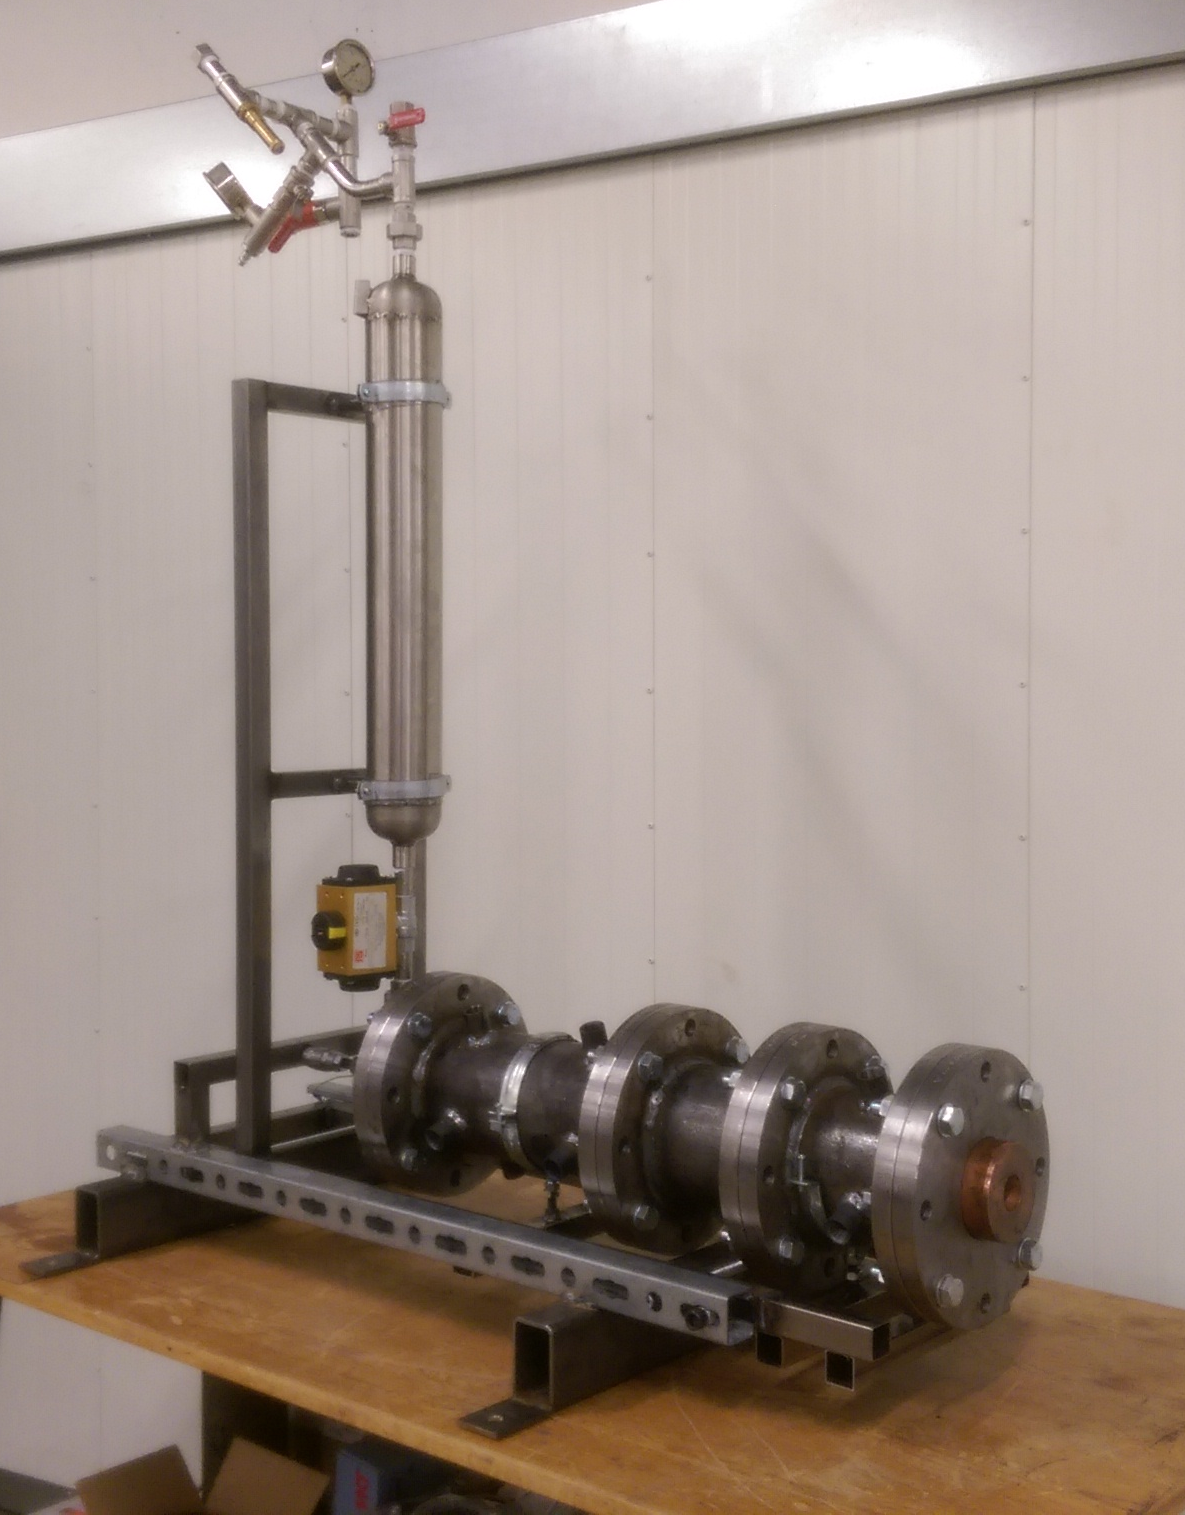
\includegraphics[width=0.5\textwidth]{rocketstand}
	\caption{The hybrid rocket build at Navitas in Aarhus for educational purposes.}
	\label{fig:rocketpic}
\end{figure}

	The hybrid rocket engine consists of three parts: The combustion chamber, the converging into a throat, and diverging section after called the nozzle. A rocket's effectivity is highly dependent on the shape, size and ratios between these three segments. Accordingly, it is imperative to study these parts of the rocket's design.

	The rocket in question is seen in figure \ref{fig:rocketpic} which is divided into a tank, three chambers and a nozzle. From the left: The tall tank contains the oxidizing agent, which is injected into the first part of the rocket. The longest part of the rocket, as seen on figure \ref{fig:rocketpic}, contains potassium permanganate engulfed in a flame retardant foam. This creates oxygen, which is forced through the rocket's second part: the grain chamber. The heat from decomposition heats the inside material to roughly 485K, which is close to MDF's autoignition point of 492K at atmospheric oxygen levels. \cite{mdfAIT} With almost pure oxygen being created in the decomposition, the autoignition temperature drops and combustion takes place. The exhaust exits through the nozzle after it has passed the mixing chamber.

	All calculations and considerations made in the report is in regard to this particular rocket. The following subsections elaborates each individual segment of the rocket, with the purpose of providing the necessary background knowledge to understand the simulations and results. The explanation is given step by step, starting with injection and ending with exhaustion.


\subsection{Injection}

	To initiate combustion in the hybrid engine, an oxidizer is injected into the combustion chamber. The rocket in question creates its oxydizer by mixing an oxidizing agent with potassium permanganate. The agent is contained in a pressurized tank containing an $80 \%$ \chem{H_2O_2} rich mixture with the remainder being \chem{H_2O}. The oxidizing agent is assumed to be injected at a constant rate of:
		\begin{align}
			\dot{m}_\text{injection} = \SI{0.273}{kg/s}.
		\end{align}
	in accordance to data collected at the recent launch \fxnote{Hvordan angiver jeg kilde/skal jeg ændre dette til at være tidsafhængig?}.

	The oxidizing agent is injected into the first chamber where decomposition into \chem{O_2} is aided by potassium permanganate. The hydrogen-peroxide (\chem{H_2O_2}) decomposes into dioxygen (\chem{O_2}) as it reacts with the potassium permanganate (\chem{K Mn O_4}), which is encased in a flame retardant foam. The unbalanced chemical reaction is as follows:
		\begin{align}
			\chem{KMnO_4 + H_2O_2} &\rightarrow \chem{K_2O_2 + MnO_2 + H_2O + O_2}
		\intertext{The specific enthalpy released during decomposition is:}
			\Delta h_\text{decomposition} &= \frac{\Delta H_\chem{H_2O_2}}{\text{M}_\chem{H_2O_2}}
		\intertext{Where $\Delta H$ is the change in enthalpy. The energy released heats the grain's surface to autoignition temperatures of approximately $\SI{260}{^\circ C}$ in this extremely oxygen-rich environment. The increased temperature increases the pressure, in accordance to the ideal-gas law:}
			P V &= n R T
		\end{align}
	The ideal gas law is crucial in our description of the rocket. Describing the rocket's upstart phase requires coupling the changes in temperature $T$, pressure $P$ and amount of substance $n$. During injection and decomposition, combustion occurs simultaneously.

\subsection{Combustion Chamber}

	The combustion chamber contains two important theoretical aspects. First, the propellant grain has significant effects on the rocket's thrust over time. Secondly, the theoretical description of the rocket's combustion allows us to estimate different working parameters, and deciding the rocket nozzle's size and area ratios.

	\subsubsection{Propellant Grain}
		The combustion chamber consists of an approximate 3 liter cavity which is filled with the grain. The actual volume in a hybrid rocket depends strongly on the initial condition of the grain and the fuel's combustion rate. Holes have to be carved in the grain to allow oxygen to reach the grain's surface, and transport exhaust towards the throat. The combustion rate is largely determined by the exposed surface area of the grain, and the flux of the oxidizer. The surface gradually expands as the outer regions are burned away, thus changing the rocket's effective thrust over time \cite[chapter 12, p.~174]{ignition}. \emph{The propellant's increase in burning area during the first second is assumed to be negligible, compared to the rapid increases in pressure and temperature.}\fxnote{Er det her en god antagelse?}

		The shapes and sizes of the holes in the grain has a large impact on the initial ignition and thrust ratios. \cite{nakka} Therefore, several different grain geometries are being tested \fxnote{SKRIV OM DE FORSKELLIGE, HVILKE HAR VI VALGT? HVORFOR?}. Depending on the surface areas, the different grain's regression rate varies greatly over time. Unless oxygen is the limiting factor, the regression rate will be proportional to the thrust. The generated thrust is directly proportional to the instantaneous burning area, and as this area increases, so does the thrust.

		An alternative explanation to the pressure spike could therefore be a very fast increase in regression area. The grain's specifications from the previous tests are not mentioned, but a wagon-wheel design with several holes could allow ignition in single canals before all of them. This could allow hot pyrolytic fuel and oxygen to accumulate, causing an eventual explosion.

	\subsubsection{Combustion}

		As temperatures reach the MDF's autoignition point, and oxygen levels increase, combustion starts taking place. The combustion reaction can be described chemically by the formula:
			\begin{align}
				\chem{C_3 H_4 O_2 + 3 O_2} &\rightarrow \chem{3 CO_2 + 2H_2O}
			\end{align}
		Energy released in this reaction heats up the chamber's fluids towards a design temperature of $\SI{2498}{K}$. Assuming a \emph{closed} chamber, the rise in temperature and amount of substance yields an exponential increase in pressure over time. This is not a desired property, as that would eventually lead to engine destruction. The accumulated decomposed and combusted material leaves through the rocket's throat, which allows the rocket to reach pressure-equilibrium. The throat's area is essential to the rocket's pressure and thus stability, hence the advance to the throat.

\subsection{Throat}

	\begin{figure}
		\includegraphics[width=\textwidth]{elon3}
		\caption{Cross section of the throat area.}
		\label{fig:crossthroat}
	\end{figure}

	The throat begins at the end of the combustion chamber, at the opposite side of where injection occurs. The throat is characterized by the convergence of the rocket chamber into a small passage called the throat, followed by a diverging section: The nozzle. The throat's cross-sectional area is what determines the maximum flow rate, as the speed of sound restricts the flow of matter. In order to calculate the amount of matter contained in the chamber, it is crucial to know how much is flowing out. Due to conservation of mass, the flow rate $\dot{m}_t$ must be proportional to the density of the material, the velocity and the throat's area:
		\begin{align}
			\dot{m}_t &= \rho \cdot v_t \cdot A_t
		\intertext{\cite{nasacompflow} The velocity $v_t$ is thus roughly proportional to the mass flow as the area and density are approximately constant in this case. Hence, as the matter approaches the speed of sound, the flow rate out of the rocket stagnates. This is called mass flow choking, which must be at a maximum when the velocity is equal to the speed of sound. This condition is satisfied when the mach number $M=1$. For an ideal compressible gas, this becomes:}
			\dot{m}_t &= \frac{A_t P_c}{\sqrt{T_t}} \sqrt{\frac{\gamma}{\text{R}}} \left(\frac{\gamma+1}{2}\right)^{-\frac{\gamma+1}{2(\gamma-1})}
		\end{align}
	Where $P_c$ is the pressure in the combustion chamber, $T_t$ is the temperature in the throat, $\gamma$ is the specific heat ratio and R is the gas constant. \cite{nasacompflow} Three outcomes are possible:
	\begin{align*}
		\dot{m}_t < \dot{m}_{in} & ~,~ \text{less mass is coming out than is flowing "into" the rocket.} \\
		\dot{m}_t = \dot{m}_{in} & ~,~ \text{mass outflow equilibrium.} \\
		\dot{m}_t > \dot{m}_{in} & ~,~ \text{more mass is flowing out than is being created.}
	\end{align*}
	The first outcome would yield increasing pressure until the rocket has burned all of it's fuel, or it explodes. The second option is what we know as a safe and steady rocket, assuming the designed mass flow equilibrium is within the rocket's boundaries. The final outcome will yield a slow decrease in pressure over time, until the rocket has been exhausted for material inside and combustion ceases. \fxnote{Passer det med masse?}

	In order to describe the initial pressure spike it is necessary to not assume any of these conditions. The abrupt change from the first to the second condition is what is hypothesized to cause the spike in pressure. Therefore, simulating the mass flow out of the rocket is essential to our understanding of the phenomenon. This does however require knowledge of several key parameters within the rocket, which are difficult to calculate, unless some things are assumed, such as conservation of entropy. However, in order to combine this knowledge, we first have to look at the final piece:

\subsection{Nozzle}

	As the fluid is pushed through the throat it is highly pressurized. The nozzle is in contact with the surroundings, which acts as a reservoir of low-pressure gas between atmospheric pressure ($\SI{101.3}{kPa}$).
	and no pressure (in space!), depending on the rocket's whereabouts. The expansion of course depends on the surrounding pressure, but in general, the plume can be over- and underexpanded and ambient. Ambient is the preferred expansion of the plume, where the exhaust gas is in pressure equilibrium with the surrounding air. If the exhaust has the same pressure as the surroundings, the gas is optimally expanded, and provides the maximum amount of thrust to the rocket.

\subsection{Isentropic Flow}

	In order to effectively describe the rocket's behavior, we have to assume a few things:
	\begin{enumerate}
		\item{Entropy is conserved.}
		\item{Decomposition and combustion products obey the perfect gas law.}
		\item{All chemical reactions are adiabatic: No heat is lost to the surroundings.}
		\item{The fluid velocity inside the chamber is approximately zero, allowing us to assume stagnated pressure. The velocity is \emph{not} assumed to be zero when entering the throat and nozzle, however.}
	\end{enumerate}

	The assumption of of isentropic flow stems from the idea that the process is reversible. The fluid will, after moving through the nozzle, have the same original values. The second law of thermodynamics states that reversible flow maintains entropy, and this allows us to calculate almost any value related to the rocket's flow. It is therefore an essential piece to the project.

	If supersonic flow is not achieved by gradual means, isentropic flow is not a valid assumption. If shock waves occur abruptly, isentropic flow is not a valid assumption. Hence, exit values are simulated before any normal or oblique shock relations occur. \cite{nasaisentrop}
